\begin{tikzpicture}
\node[draw,text width=17cm, line width=0.5mm, rounded corners=10pt, fill=yellow!50] at (0,0) % rounded rectangle
{
\begin{itemize}
\section*{\colorbox{black}{\textcolor{white}{\bf Specification CCEA Yr. 11 DA Science:}}}
    \item[\bf M1] {\bf Investigate and	use	the	quantitative	relationships between initial	speed, final speed, average speed, distance	moved, rate	of change of speed and time.}
    \item[\bf M2] {\bf calculate the	average	speed from linear distance–time graphs.}
    \item[\bf M3] {\bf define that	distance	is	measured	in	metres	(m), speed	in	metres	per	second	(m/s)	and	rate	of change	of	speed	in	metres	per	second	squared	(m/s$^2$).}
    \item[\bf M4] {\bf Recall and use the equations:
        \begin{equation*}
        \begin{split}
            & \text{Average speed}=\frac{\text{distance moved}}{\text{time taken}}\hspace{0.5cm}\text{or}\hspace{0.5cm}v=\frac{s}{t}\\
            & \text{Average speed}=\frac{\text{initial speed+final speed}}{2}\hspace{0.5cm}\text{or}\hspace{0.5cm}v=\frac{v_\text{i}+v_\text{f}}{2}\\
            &\text{Rate of change of speed}=\frac{\text{final speed-initial speed}}{\text{time taken}}\hspace{0.5cm}\text{or}\hspace{0.5cm}v=\frac{v_\text{f}-v_\text{i}}{t}\\
        \end{split}
        \end{equation*}
    }
    \item[\textcolor{GREEN}{\bf M5}] \textcolor{GREEN}{\bf \underline{Prescribed Practical P1:} use simple apparatus, including	trolleys,	ball-bearings, metre rules,	stop-clocks	and	ramps to investigate experimentally	how	the	average	speed of an	object moving	down a runway depends on the slope of the	runway	measured as the	height	of one end	of the runway (ICT	resources could	be used to	process	the	measurements and analyse the data).}
    \vspace{10mm}
\end{itemize}
};
\end{tikzpicture} 
%
%
\thispagestyle{empty}

%
\newpage

%
%
\begin{tikzpicture}
\node[draw,text width=17cm, line width=0.5mm, rounded corners=10pt, fill=yellow!50] at (0,0) % rounded rectangle
{
\begin{itemize}
\section*{Specification CCEA Yr11-Physics:}
    \item[\bf M6] {\bf demonstrate	understanding that:
    \begin{itemize}
        \item[\bf (a)] A vector is a quantity that depends on	direction and scalar	is a quantity that does	not.
        \item[\bf (b)] displacement	is	a	vector	and	that	distance	is	a	scalar	but	both	are	measured	in	metres	(m).
        \item[\bf (c)] velocity	is	a vector	and	speed is scalar but	both are measured in	metres per second (m/s).
        \item[\bf (d)] Acceleration	is a	vector	and	rate of	change of speed is	a	scalar	but	both	are	measured in metres	per	second	squared	(m/s$^2$).
    \end{itemize}
    }
    \item[\bf M7] {\bf Recall and use the	quantitative relationships between displacement, time and average velocity:
    \begin{equation*}
        \text{Average velocity}=\frac{\text{displacement}}{\text{time taken}}\hspace{0.5cm}\text{or}\hspace{0.5cm}\vec{v}=\frac{\vec{d}}{t}
    \end{equation*}
    }
    \item[\bf M8] {\bf Recall and use the	quantitative relationships between initial	velocity, final velocity,	acceleration and time:
    \begin{equation*}
        \text{Average velocity}=\frac{\text{initial velocity+final velocity}}{2}\hspace{0.5cm}\text{or}\hspace{0.5cm}\vec{v}=\frac{\vec{v}_\text{i}+\vec{v}_\text{f}}{2}
    \end{equation*}
    }
    \item[\bf M9] {\bf Recall and use the	quantitative relationships between initial	velocity, final velocity,	acceleration and time:
     \begin{equation*}
         \text{Acceleration}=\frac{\text{final velocity-initial velocity}}{\text{time taken}}\hspace{0.5cm}\text{or}\hspace{0.5cm}\vec{a}=\frac{\vec{v}_\text{f}-\vec{v}_\text{i}}{t}
     \end{equation*}
     }
     \item[\bf M10] {\bf Explain that	negative acceleration is called retardation.}
     \item[\bf M11] {\bf Use graphical methods to determine speed, distance	and	rate of change of speed, applying knowledge that:
     \begin{itemize}
         \item[\bf (a)] The	slope of a distance-time	graph is the speed
         \item[\bf (b)] The slope of	a speed–time graph is the	rate of change of speed.
         \item[\bf (c)] The	area	under a speed-time graph	is the distance moved.
     \end{itemize}	
     }
    \vspace{10mm}
\end{itemize}
};
\end{tikzpicture} 
     \newpage

%
%
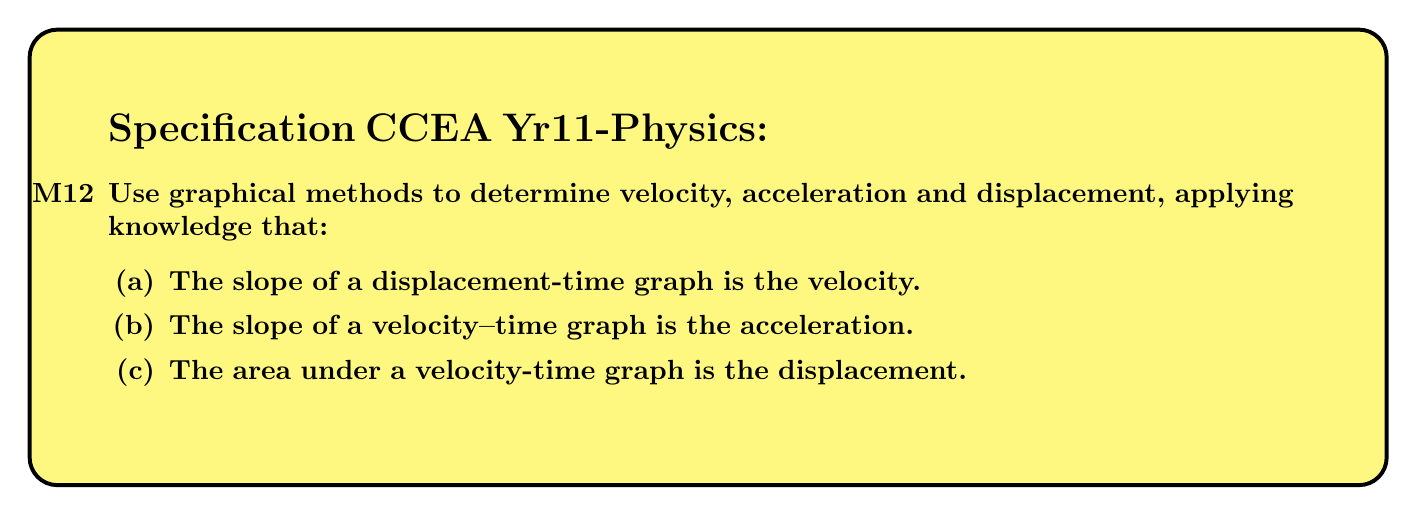
\begin{tikzpicture}
\node[draw,text width=17cm, line width=0.5mm, rounded corners=10pt, fill=yellow!50] at (0,0) % rounded rectangle
{
\begin{itemize}
\section*{Specification CCEA Yr11-Physics:}
     \item[\bf M12] {\bf Use graphical methods to determine velocity, acceleration and	displacement, applying knowledge that:
     \begin{itemize}
         \item[\bf (a)] The	slope	of a displacement-time	graph is the velocity.
         \item[\bf (b)] The	slope of a velocity–time	graph is the acceleration.
         \item[\bf (c)] The area under a velocity-time graph is the displacement.
     \end{itemize}	
     }
    \vspace{10mm}
\end{itemize}
};
\end{tikzpicture} 
%
%
%
%
%
%
%
%
\newpage